\documentclass[10pt]{article}
\usepackage[margin=0.68in]{geometry}
\usepackage{graphicx,booktabs,amsmath,hyperref,microtype,tikz,float}
\usetikzlibrary{arrows.meta,positioning}
\setlength{\parindent}{0pt}\setlength{\parskip}{4pt}
\title{\vspace{-1.4cm}AI Agent for Multimodal Representation Learning}
\author{Cassi Chen}\date{}
\begin{document}\maketitle\vspace{-0.8cm}

\section{Introduction and Overview of System Architecture}

Multimodal representation learning for biomedical data requires decisions for preprocessing, model selection, hyperparameters, evaluation, 
and interpretation. Unlike a traditional benchmarking study, this project develops an AI agent that automatically 
determines how multiple data modalities should be integrated to learn meaningful joint representations 
for downstream analysis with minimal human guidance. Given a dataset and a user-specified objective, 
the agent determines an appropriate multimodal representation learning workflow, trains suitable models, 
evaluates the learned representations and performs downstream analysis, all autonomously.

The overall agent design in this project was inspired by the UNC BIOS 774 course Lecture 9 slides \cite{bios774slides}. 
Figure~\ref{fig:architecture} summarizes the workflow for this project. Specifically, the researcher specifies the dataset and analysis objective, local Python programs perform deterministic 
computations, and the LLM recovers context, invokes code, and interprets the results against to the task. 
The researcher launches the workflow through a single command with \texttt{run\_agent.py}. 

\begin{figure}[H]
    \centering
    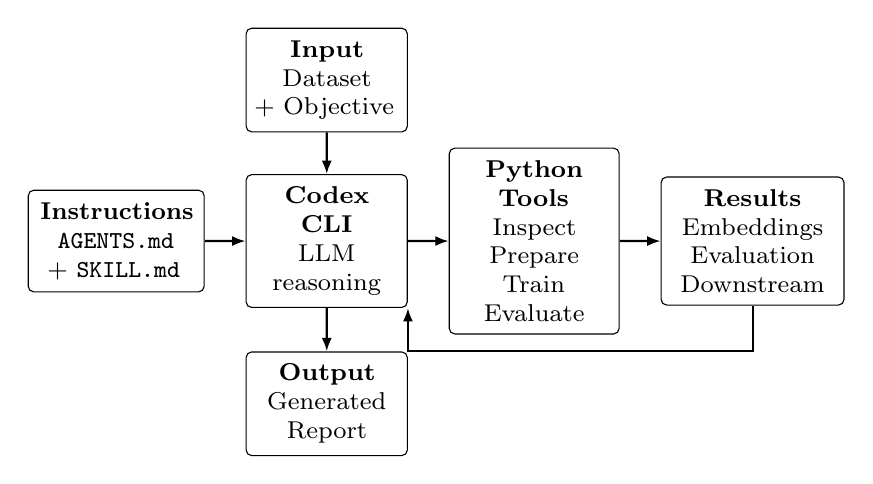
\begin{tikzpicture}[
        scale=1.1,
        transform shape,
        box/.style={
            draw,
            rounded corners=2pt,
            align=center,
            font=\footnotesize,
            inner sep=4pt,
            minimum height=0.65cm
        },
        arr/.style={-{Latex[length=1.7mm]}, thick},
        node distance=0.45cm and 0.47cm
    ]
    % Instructions
    \node[box, text width=1.75cm] (instructions) {
        \textbf{Instructions}\\
        \texttt{AGENTS.md}\\
        + \texttt{SKILL.md}
    };
    % Agent
    \node[box, text width=1.58cm, right=of instructions] (agent) {
        \textbf{Codex CLI}\\
        LLM reasoning
    };
    % Python tools
    \node[box, text width=1.68cm, right=of agent] (tools) {
        \textbf{Python Tools}\\
        Inspect\\
        Prepare\\
        Train\\
        Evaluate
    };
    % Results
    \node[box, text width=1.83cm, right=of tools] (results) {
        \textbf{Results}\\
        Embeddings\\
        Evaluation\\
        Downstream
    };
    % Input
    \node[box, above=0.48cm of agent, text width=1.58cm] (data) {
        \textbf{Input}\\
        Dataset\\
        + Objective
    };
    % Report
    \node[box, below=0.50cm of agent, text width=1.58cm] (report) {
        \textbf{Output}\\
        Generated Report
    };
    % Arrows
    \draw[arr] (instructions) -- (agent);
    \draw[arr] (data) -- (agent);
    \draw[arr] (agent) -- (tools);
    \draw[arr] (tools) -- (results);
    \draw[arr] (agent) -- (report);
    % Feedback from results to agent
    \draw[arr]
        (results.south) -- ++(0,-0.52)
        -| (agent.south east);

    \end{tikzpicture}
    \caption{Agent architecture.}
    \label{fig:architecture}
\end{figure}

\section{Agent Decision-Making and Implementation}

The agent begins by invoking the \texttt{inspect\_raw.py} tool to characterize modality structure, 
such as sample counts, sparsity, and missingness. Based on these details, the LLM selects dataset-specific 
preprocessing methods using \texttt{prepare\_dataset\_1.py} or \texttt{prepare\_dataset\_2.py}. 
\texttt{inspect\_data.py} then verifies that the preprocessed features are valid and that paired samples remain correctly
aligned across the training, validation, and test splits. 

After preprocessing, the LLM considers all available representation learning methods. 
It proposes three method--encoder candidates per dataset. 
The \texttt{train.py} tool trains each candidate, the \texttt{evaluate.py} tool assesses representation quality 
with metrics such as pairwise AUC, cosine similarity gap, alignment, and effective rank,
and the \texttt{downstream.py} tool evaluates cross-modal retrieval performance 
with metrics such as Recall@K, mean reciprocal rank, and median rank. 
The agent then selects the candidate with the highest mean 
bidirectional Recall@5. It is then evaluated on the held-out test split 
using both \texttt{evaluate.py} 
and \texttt{downstream.py}, producing final representation-quality metrics 
and downstream retrieval results. Model configurations and training histories are saved.

The main tools and AI models used in this project are provided
in Table~\ref{tab:tools}.

\begin{table}[H]
    \centering
    \small
    \begin{tabular}{@{}p{3.5cm}p{1.8cm}p{10.0cm}@{}}
        \toprule
        \textbf{Component} & \textbf{Type} & \textbf{Role} \\
        \midrule
        Codex CLI & AI Model &
        Tool selection, model decisions, interpretation, and reporting \\

        \texttt{inspect\_raw.py} & Tool &
        Raw dataset inspection \\

        \texttt{inspect\_data.py} & Tool &
        Preprocessed feature inspection and split alignment \\

        \texttt{prepare\_dataset\_1.py} & Tool &
        ROCOv2 image--text preprocessing \\

        \texttt{prepare\_dataset\_2.py} & Tool &
        Multiome RNA--ATAC preprocessing \\

        \texttt{train.py} & Tool &
        Candidate representation-model training \\

        \texttt{evaluate.py} & Tool &
        Embedding-quality evaluation and diagnostics \\

        \texttt{downstream.py} & Tool &
        Cross-modal retrieval evaluation \\

        \bottomrule
    \end{tabular}
    \caption{Agent tools and AI models.}
    \label{tab:tools}
\end{table}

\section{Experimental Results}

The system was evaluated on two multimodal biomedical datasets: ROCOv2, 
containing paired medical images and text reports, and 10x Multiome, 
containing paired RNA and ATAC measurements from individual cells. 
Data-dependent preprocessing was performed on each dataset. Each dataset was also divided 
into training, validation, and held-out test splits. Model training was performed using MPS acceleration.

In the following subsections, quantitative results focus on the quality of the 
learned multimodal representations and their downstream cross-modal retrieval 
performance. Validation data were used to select the best candidate based on mean 
bidirectional Recall@5, while the held-out test data were used only for final evaluation.

\subsection{ROCOv2: Radiology Images and Text Reports}

The agent sampled 8,000 training pairs and 1,000 
validation pairs from the official ROCOv2 training split, with 1,000 held-out test pairs sampled from the official 
validation split. Each pair contained image and report data. 

During preprocessing, a frozen ImageNet-pretrained ResNet18 extracted 512 image features
and training-fitted TF-IDF (unigrams and bigrams) followed with truncated SVD extracted 128 report 
features. 

The agent chose contrastive learning with 64-dimensional embeddings, 
batch size 128, and 25 epochs. The agent selected contrastive learning because the objective was to align paired 
image and text representations for cross-modal retrieval. 
Although ROCOv2 provides medical concept annotations, these labels 
were not used in the experiment. Supervised learning was therefore not pursued,
while self-supervised reconstruction was less directly aligned with the cross-modal 
retrieval objective. Table~\ref{tab:roco} shows the three contrastive encoder 
configurations considered, all trained using a symmetric InfoNCE loss.


\begin{table}[H]
\centering\small\setlength{\tabcolsep}{7pt}
\begin{tabular}{lccc}
\toprule
\textbf{Image / text encoder} & \textbf{Image$\to$text R@5} & \textbf{Text$\to$image R@5} & \textbf{Mean R@5}\\\midrule
Linear / Linear (selected) & 16.6\% & 14.1\% & \textbf{15.35\%}\\
MLP / Linear & 12.0\% & 11.6\% & 11.80\%\\
MLP / MLP & 12.4\% & 12.2\% & 12.30\%\\\bottomrule
\end{tabular}
\caption{ROCOv2 validation retrieval among 1,000 paired candidates.}
\label{tab:roco}
\end{table}

A contrastive linear/Linear encoder produced the highest mean R@5. 
Thus, it was selecetd as the encoder configation for the test data. 

Table~\ref{tab:test-summary} summarizes the results for representation quality. 
For ROCOv2, the selected model achieved a pairwise AUC of 0.9024, 
indicating that matched image--caption pairs generally received higher 
similarity scores than unmatched pairs. 

Table~\ref{tab:retrieval} summarizes the results for downstream quality. 
Mean bidirectional Recall@K increased from 3.70\% at K=1 to 13.70\% at K=5, 
23.55\% at K=10, 56.00\% at K=50, and 73.30\% at K=100. These values 
consistently exceeded the corresponding random baselines of 0.10\%, 0.50\%, 1.00\%, 
5.00\%, and 10.00\%, respectively. In summary, the learned representations 
ranked matching image--report pairs substantially better than random retrieval.

Not that neither retrieval nor pairwise AUC alone establishes clinical validity. This is because although the test embeddings exhibit positive-pair separation,
the exact top-1 retrival remains low. 

\subsection{Multiome: Single-cell RNA-seq and ATAC-seq}

The original 10x Multiome dataset contained 10,970 paired cells, of which 
8,776 were used for training, 1,097 for validation, and 1,097 for held-out 
testing. Each cell contained paired RNA and ATAC data.

During preprocessing, RNA counts were normalized to 10,000 counts per cell and 
log-transformed, with 2,000 highly variable genes selected using the training data. 
ATAC counts were binarized and transformed using TF-IDF, with 12,000 peaks selected 
from the training data. Truncated SVD then reduced each modality to 64 features. 

The agent considered contrastive learning and self-supervised reconstruction. 
Contrastive learning was favored because the dataset contains paired RNA and ATAC 
measurements, and the objective was to align representations across modalities. 
Supervised learning was not pursued because cell-type labels were not used in the 
experiment. The agent proposed 32-dimensional embeddings, a batch size of 256, and 
30 training epochs. The contrastive candidates minimized a symmetric InfoNCE loss, 
while the self-supervised candidate minimized a reconstruction loss. 
Table~\ref{tab:multiome} shows the three candidate configurations.

\begin{table}[H]
\centering\small\setlength{\tabcolsep}{7pt}
\begin{tabular}{lccc}
\toprule
\textbf{Method; RNA / ATAC} & \textbf{RNA$\to$ATAC R@5} & \textbf{ATAC$\to$RNA R@5} & \textbf{Mean R@5}\\\midrule
Contrastive; linear / linear (selected) & 8.93\% & 7.47\% & \textbf{8.204\%}\\
Contrastive; MLP / MLP & 8.57\% & 6.47\% & 7.521\%\\
Self-supervised; MLP / linear & 0.456\% & 0.365\% & 0.410\%\\\bottomrule
\end{tabular}
\caption{Multiome validation retrieval among 1,097 paired candidates.}
\label{tab:multiome}
\end{table}

A contrastive linear/Linear encoder produced the highest mean R@5. 
Thus, it was selecetd as the encoder configation for the test data. 

Table~\ref{tab:test-summary} summarizes the results for representation quality. F
or Multiome, the selected model achieved a pairwise AUC of 0.9015, 
indicating that matched RNA--ATAC pairs generally received higher similarity 
scores than unmatched pairs.

Table~\ref{tab:retrieval} summarizes the results for downstream quality. 
Mean bidirectional Recall@K increased from 2.64\% at K=1 to 9.03\% at K=5, 
15.36\% at K=10, 43.71\% at K=50, and 63.04\% at K=100. 
These values consistently exceeded the corresponding random baselines 
of 0.091\%, 0.456\%, 0.912\%, 4.558\%, and 9.116\%, respectively. In summary, 
the learned representations ranked matching RNA--ATAC pairs substantially better 
than random retrieval.

\begin{table}[H]
\centering\small\setlength{\tabcolsep}{5pt}
\begin{tabular}{lcc}
\toprule
\textbf{Test representation-quality metric} & \textbf{ROCOv2} & \textbf{Multiome}\\\midrule
Mean matched / nonmatched cosine & 0.3288 / 0.0019 & 0.5486 / 0.0506\\
Cosine similarity gap & 0.3269 & 0.4980\\
Positive-vs-negative pairwise AUC & 0.9024 & 0.9015\\
Alignment (mean squared distance) & 1.3424 & 0.9028\\
Uniformity (modality 1 / modality 2) & $-3.7224$ / $-3.6294$ & $-2.5349$ / $-2.3924$\\
Effective rank (modality 1 / modality 2) & 45.10 / 42.90 (of 64) & 9.89 / 9.20 (of 32)\\
\bottomrule
\end{tabular}
\caption{\texttt{evaluate.py}: representation quality of the \emph{selected model on held-out test data}. Modalities are image/text for ROCOv2 and RNA/ATAC for Multiome.}
\label{tab:test-summary}
\end{table}

\begin{table}[H]
\centering\small\setlength{\tabcolsep}{5pt}
\begin{tabular}{lcccc}
\toprule
 & \multicolumn{2}{c}{\textbf{ROCOv2 test}} & \multicolumn{2}{c}{\textbf{Multiome test}}\\
\textbf{Retrieval metric} & \textbf{Mean} & \textbf{Random} & \textbf{Mean} & \textbf{Random}\\\midrule
Recall@1 & 3.70\% & 0.10\% & 2.64\% & 0.091\%\\
Recall@5 & 13.70\% & 0.50\% & 9.03\% & 0.456\%\\
Recall@10 & 23.55\% & 1.00\% & 15.36\% & 0.912\%\\
Recall@20 & 35.15\% & 2.00\% & 24.48\% & 1.823\%\\
Recall@50 & 56.00\% & 5.00\% & 43.71\% & 4.558\%\\
Recall@100 & 73.30\% & 10.00\% & 63.04\% & 9.116\%\\
Mean reciprocal rank & 0.1024 & --- & 0.0726 & ---\\
Mean directional median rank & 38.5 & --- & 64 & ---\\
\bottomrule
\end{tabular}
\caption{\texttt{downstream.py}: bidirectional exact-pair retrieval on held-out test data (1,000 ROCOv2 pairs; 1,097 Multiome cells). Random Recall@K equals $K/N$. These are distinct retrieval tasks and gallery sizes.}
\label{tab:retrieval}
\end{table}

Not that neither retrieval nor pairwise AUC alone establishes biological validity. This is because although the test embeddings exhibit positive-pair separation,
the exact top-1 retrival remains low. 



\section{Strengths, Limitations, and Conclusion}

The main strength of the system is that entire process is autonomously done by an agent. 
The two tests conducted on ROCOv2 and Multiome also show that the agent is able to adapt across 
different data modalities. 

The system also has many limitations. One is that the agent can only choose among the supplied preprocessing 
and learning representation models. Another is that preprocessing and learning representation model methods and hyperparameter selection rely solely on LLM (Codex CLI) reasoning instead of a specified criteria. 

Overall, this project showcases an AI agent that automatically performs learning representation modeling while maintaining reproducibility.


\begin{thebibliography}{9}
\bibitem{bios774slides} Longfei Zhang. \textit{BIOS 774 Course Slides: An Intro to Building Agents in 2026}. 2026.
\bibitem{rocov2} Johannes Rückert et al. \textit{ROCOv2: Radiology Objects in COntext Version 2, An Updated Multimodal Image Dataset}. Version 2.0 [Dataset]. Zenodo, 2023. \url{https://doi.org/10.5281/zenodo.8333645}.
\bibitem{multiome} 10x Genomics. \textit{10k Human PBMCs, Multiome v1.0, Chromium X}. 2021. \url{https://www.10xgenomics.com/datasets/10-k-human-pbm-cs-multiome-v-1-0-chromium-x-1-standard-2-0-0}.
\end{thebibliography}
\end{document}
